\documentclass[border=5pt]{standalone}
\usepackage{amssymb}
\usepackage{tikz}
\usetikzlibrary{positioning, arrows.meta, patterns, calc}
\begin{document}
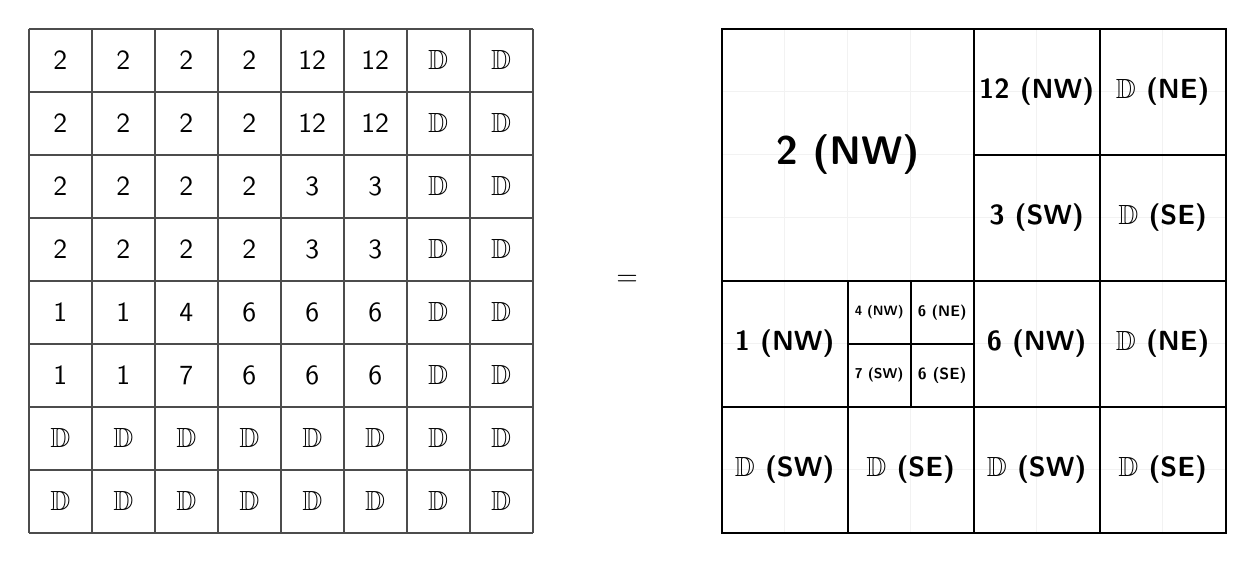
\begin{tikzpicture}[
    scale=0.8,
    font=\sffamily,
    % one style per block size: font is declared once, in sans serif
    big/.style   = {midway, font=\sffamily\Large\bfseries},
    med/.style   = {midway, font=\sffamily\bfseries},
    small/.style = {midway, inner sep=0pt},
    block/.style = {draw=black, thick},
  ]

  %% ---------- left: the dense 8x8 matrix ----------
  \draw[step=1cm, black!70, thick] (0,0) grid (8,8);

  \foreach \x/\y/\val in {
    0/0/$\mathbb{D}$, 1/0/$\mathbb{D}$, 2/0/$\mathbb{D}$, 3/0/$\mathbb{D}$, 4/0/$\mathbb{D}$, 5/0/$\mathbb{D}$, 6/0/$\mathbb{D}$, 7/0/$\mathbb{D}$,
    0/1/$\mathbb{D}$, 1/1/$\mathbb{D}$, 2/1/$\mathbb{D}$, 3/1/$\mathbb{D}$, 4/1/$\mathbb{D}$, 5/1/$\mathbb{D}$, 6/1/$\mathbb{D}$, 7/1/$\mathbb{D}$,
    0/2/1, 1/2/1, 2/2/7, 3/2/6, 4/2/6, 5/2/6, 6/2/$\mathbb{D}$, 7/2/$\mathbb{D}$,
    0/3/1, 1/3/1, 2/3/4, 3/3/6, 4/3/6, 5/3/6, 6/3/$\mathbb{D}$, 7/3/$\mathbb{D}$,
    0/4/2, 1/4/2, 2/4/2, 3/4/2, 4/4/3, 5/4/3, 6/4/$\mathbb{D}$, 7/4/$\mathbb{D}$,
    0/5/2, 1/5/2, 2/5/2, 3/5/2, 4/5/3, 5/5/3, 6/5/$\mathbb{D}$, 7/5/$\mathbb{D}$,
    0/6/2, 1/6/2, 2/6/2, 3/6/2, 4/6/12, 5/6/12, 6/6/$\mathbb{D}$, 7/6/$\mathbb{D}$,
    0/7/2, 1/7/2, 2/7/2, 3/7/2, 4/7/12, 5/7/12, 6/7/$\mathbb{D}$, 7/7/$\mathbb{D}$
  } {
    \node at (\x+0.5, \y+0.5) {\val};
  }

  \node at (9.5, 4) {$=$};

  %% ---------- right: the quad-tree block decomposition ----------
  \begin{scope}[shift={(11,0)}]
    \draw[step=1cm, gray!10, very thin] (0,0) grid (8,8);

    \draw[block] (0,4) rectangle ++(4,4) node[big] {2 (NW)};
    \draw[block] (0,2) rectangle ++(2,2) node[med] {1 (NW)};

    % 1x1 cells: value and quadrant stacked so the label fits inside the cell
    \draw[block] (2,3) rectangle ++(1,1) node[small] {\resizebox{0.62cm}{!}{\sffamily\bfseries 4 (NW)}};
    \draw[block] (3,3) rectangle ++(1,1) node[small] {\resizebox{0.62cm}{!}{\sffamily\bfseries 6 (NE)}};
    \draw[block] (2,2) rectangle ++(1,1) node[small] {\resizebox{0.62cm}{!}{\sffamily\bfseries 7 (SW)}};
    \draw[block] (3,2) rectangle ++(1,1) node[small] {\resizebox{0.62cm}{!}{\sffamily\bfseries 6 (SE)}};

    \draw[block] (0,0) rectangle ++(2,2) node[med] {$\mathbb{D}$ (SW)};
    \draw[block] (2,0) rectangle ++(2,2) node[med] {$\mathbb{D}$ (SE)};

    \draw[block] (4,6) rectangle ++(2,2) node[med] {12 (NW)};
    \draw[block] (6,6) rectangle ++(2,2) node[med] {$\mathbb{D}$ (NE)};
    \draw[block] (4,4) rectangle ++(2,2) node[med] {3 (SW)};
    \draw[block] (6,4) rectangle ++(2,2) node[med] {$\mathbb{D}$ (SE)};

    \draw[block] (4,2) rectangle ++(2,2) node[med] {6 (NW)};
    \draw[block] (6,2) rectangle ++(2,2) node[med] {$\mathbb{D}$ (NE)};
    \draw[block] (4,0) rectangle ++(2,2) node[med] {$\mathbb{D}$ (SW)};
    \draw[block] (6,0) rectangle ++(2,2) node[med] {$\mathbb{D}$ (SE)};
  \end{scope}
\end{tikzpicture}
\end{document}
